%\VignetteIndexEntry{Introduction to the dataRetrieval package}
%\VignetteDepends{}
%\VignetteSuggests{}
%\VignetteImports{}
%\VignettePackage{}

\documentclass[a4paper,11pt]{article}

\usepackage{amsmath}
\usepackage{times}
\usepackage{hyperref}
\usepackage[numbers, round]{natbib}
\usepackage[american]{babel}
\usepackage{authblk}
\renewcommand\Affilfont{\itshape\small}
\usepackage{Sweave}
\renewcommand{\topfraction}{0.85}
\renewcommand{\textfraction}{0.1}
\usepackage{graphicx}


\textwidth=6.2in
\textheight=8.5in
\parskip=.3cm
\oddsidemargin=.1in
\evensidemargin=.1in
\headheight=-.3in

%------------------------------------------------------------
% newcommand
%------------------------------------------------------------
\newcommand{\scscst}{\scriptscriptstyle}
\newcommand{\scst}{\scriptstyle}
\newcommand{\Robject}[1]{{\texttt{#1}}}
\newcommand{\Rfunction}[1]{{\texttt{#1}}}
\newcommand{\Rclass}[1]{\textit{#1}}
\newcommand{\Rpackage}[1]{\textit{#1}}
\newcommand{\Rexpression}[1]{\texttt{#1}}
\newcommand{\Rmethod}[1]{{\texttt{#1}}}
\newcommand{\Rfunarg}[1]{{\texttt{#1}}}

\begin{document}
\Sconcordance{concordance:dataRetrieval.tex:dataRetrieval.Rnw:%
1 126 1 49 0 1 7 15 1 1 14 55 1 3 0 36 1 2 0 11 1 24 %
0 24 1 3 0 23 1 3 0 6 1 7 0 18 1 3 0 25 1 1 0 17 1 9 %
0 6 1 7 0 21 1 8 0 16 1 2 0 11 1 23 0 21 1 9 0 20 1 3 %
0 6 1 17 0 27 1 6 0 11 1 9 0 15 1 20 0 21 1 4 0 21 1 %
4 0 17 1 7 0 22 1 8 0 19 1 4 0 9 1 4 0 78 1 1 2 9 1 1 %
4 4 1 20 0 44 1 4 0 32 1 4 0 21 1 4 0 21 1 37 0 13 1 %
9 0 95 1 4 0 9 1 12 0 13 1 4 0 14 1 4 0 5 1 4 0 23 1 %
18 0 8 1 4 0 55 1}


%------------------------------------------------------------
\title{Introduction to the dataRetrieval package}
%------------------------------------------------------------
\author[1]{Laura De Cicco}
\author[1]{Robert Hirsch}
\affil[1]{United States Geological Survey}



\maketitle
\tableofcontents

%------------------------------------------------------------
\section{Introduction to dataRetrieval}
%------------------------------------------------------------ 
The dataRetrieval package was created to simplify the process of getting hydrologic data in the R enviornment. It has been specifically designed to work seamlessly with the EGRET package: Exploration and Graphics for RivEr Trends (EGRET). See: \url{https://github.com/USGS-R/EGRET/wiki} for information on EGRET.

There is a plethora of hydrological data available on the web. This package is designed specifically to load United States Geological Survey (USGS) hydrologic data to the R enviornment. This includes daily values, real-time (unit values), site information, and water quality sample data. 

%------------------------------------------------------------ 
\section{Getting Started}
%------------------------------------------------------------ 
This section describes the options for downloading and installing the dataRetrieval package.
%------------------------------------------------------------
\subsection{New to R?}
%------------------------------------------------------------ 
If you are new to R, you will need to first install the latest version of R, which can be found here: \url{http://www.r-project.org/}.

There are many options for running and editing R code, one nice enviornment to learn R is RStudio. RStudio can be downloaded here: \url{http://rstudio.org/}. Once R and RStudio are installed, the dataRetrieval package needs to be installed as described in the next section.

%------------------------------------------------------------
\subsection{R User: Installing dataRetrieval from downloaded binary}
%------------------------------------------------------------ 
The latest dataRetrieval package build is available for download at \url{https://github.com/USGS-R/dataRetrieval/blob/master/dataRetrieval_1.2.1.tar.gz}.  If the package's tar.gz file is saved in R's working directory, then the following command will fully install the package:

\begin{Schunk}
\begin{Sinput}
> install.packages("dataRetrieval_1.2.1.tar.gz", 
+                  repos=NULL, type="source")
\end{Sinput}
\end{Schunk}

If the downloaded file is stored in an alternative location, include the path in the install command.  A Windows example looks like this (notice the direction of the slashes, they are in the opposite direction that Windows normally creates paths):

\begin{Schunk}
\begin{Sinput}
> install.packages(
+   "C:/RPackages/Statistics/dataRetrieval_1.2.1.tar.gz", 
+   repos=NULL, type="source")
\end{Sinput}
\end{Schunk}

A Mac example looks like this:

\begin{Schunk}
\begin{Sinput}
> install.packages(
+   "/Users/userA/RPackages/Statistic/dataRetrieval_1.2.1.tar.gz", 
+   repos=NULL, type="source")
\end{Sinput}
\end{Schunk}

It is a good idea to re-start the R enviornment after installing the package, especially if installing an updated version (that is, restart RStudio). Some users have found it necessary to delete the previous version's package folder before installing newer version of dataRetrieval. If you are experiencing issues after updating a package, trying deleting the package folder - the default location for Windows is something like this: C:/Users/userA/Documents/R/win-library/2.15/dataRetrieval, and the default for a Mac: /Users/userA/Library/R/2.15/library/dataRetrieval. Then, re-install the package using the directions above. Moving to CRAN should solve this problem.

After installing the package, you need to open the library each time you re-start R.  This is done with the simple command:
\begin{Schunk}
\begin{Sinput}
> library(dataRetrieval)
\end{Sinput}
\end{Schunk}
Using RStudio, you could alternatively click on the checkbox for dataRetrieval in the Packages window.

%------------------------------------------------------------
\subsection{R Developers: Installing dataRetrieval from gitHub}
%------------------------------------------------------------
Alternatively, R-developers can install the latest version of dataRetrieval directly from gitHub using the devtools package.  devtools is available on CRAN.  Simpley type the following commands into R to install the latest version of dataRetrieval available on gitHub.  Rtools (for Windows) and latex tools are required.

\begin{Schunk}
\begin{Sinput}
> library(devtools)
> install_github("dataRetrieval", "USGS-R")
\end{Sinput}
\end{Schunk}
To then open the library, simply type:

\begin{Schunk}
\begin{Sinput}
> library(dataRetrieval)
\end{Sinput}
\end{Schunk}

\newpage
%------------------------------------------------------------
\section{Raw Data: USGS Web Retrieval Examples}
%------------------------------------------------------------ 
In this section, we will run through 5 examples, documenting how to get raw data from the web. This includes historical daily values, real-time current values, water quality data, site information, and measured parameter information. 
%------------------------------------------------------------
\subsection{USGS Web Retrieval Introduction}
%------------------------------------------------------------
The United States Geological Survey organizes their hydrological data in fairly standard structure.  Gage stations are located throughout the United States, each station has a unique ID.  Often (but not always), these ID's are 8 digits.  The first step to finding data is discoving this 8-digit ID. One potential tool for discovering data is Environmental Data Discovery and Transformation (EnDDaT): \url{http://cida.usgs.gov/enddat/}.  Follow the example in the User's Guide to learn how to discover USGS stations and available data from any location in the United States. Essentially, you can create a Project Location on the map, set a bounding box (in miles), then search for USGS Time Series and USGS Water Quality Data. Locations, ID's, available data, and available time periods will load on the map and appropriate tabs.

Once the site-ID is known, the next required input for USGS data retrievals is the 'parameter code'.  This is a 5-digit code that specifies what measured paramater is being requested.  A complete list of possible USGS parameter codes can be found here: 

\url{http://nwis.waterdata.usgs.gov/usa/nwis/pmcodes?radio_pm_search=param_group&pm_group=All+--+include+all+parameter+groups&pm_search=&casrn_search=&srsname_search=&format=html_table&show=parameter_group_nm&show=parameter_nm&show=casrn&show=srsname&show=parameter_units}

Not every station will measure all parameters. The following is a list of commonly measured parameters:

% latex table generated in R 2.15.2 by xtable 1.7-0 package
% Wed Jan 23 10:35:45 2013
\begin{table}[ht]
\begin{center}
\caption{Commonly found USGS Parameter Codes}
\begin{tabular}{rll}
  \hline
 & pCode & shortName \\ 
  \hline
1 & 00060 & Discharge [cfs] \\ 
  2 & 00065 & Gage height [ft] \\ 
  3 & 00010 & Temperature [C] \\ 
  4 & 00045 & Precipitation [in] \\ 
  5 & 00400 & pH \\ 
   \hline
\end{tabular}
\end{center}
\end{table}
For real-time data, the parameter code and site ID will suffice.  The USGS stores historical data as daily values however.  The statistical process used to store the daily data is the final requirement for daily value retrievals.  A 5-digit 'stat code' specifies the requested processing.  A complete list of possible USGS stat codes can be found here:

\url{http://nwis.waterdata.usgs.gov/nwis/help/?read_file=stat&format=table}

The most common stat codes are:
% latex table generated in R 2.15.2 by xtable 1.7-0 package
% Wed Jan 23 10:35:45 2013
\begin{table}[ht]
\begin{center}
\caption{Commonly found USGS Stat Codes}
\begin{tabular}{rll}
  \hline
 & StatCode & shortName \\ 
  \hline
1 & 00001 & Maximum \\ 
  2 & 00002 & Minimum \\ 
  3 & 00003 & Mean \\ 
  4 & 00008 & Median \\ 
   \hline
\end{tabular}
\end{center}
\end{table}

We will use the Choptank River near Greensboro, MD as an example.  The site-ID for this gage station is 01491000. Daily discharge measurements are available as far back as 1948.  Additionally, forms of nitrate and nitrogen have been measured dating back to 1964.

%------------------------------------------------------------
\subsection{USGS Daily Value Retrievals}
%------------------------------------------------------------
To obtain historic daily records of USGS data, use the retrieveNWISData function. The arguments for this function are siteNumber, parameterCd, startDate, endDate, statCd, and a logical (true/false) interactive. There are 2 default argument: statCd defaults to "00003" and interactive defaults to TRUE.  If you want to use the default values, you do not need to list them in the function call. Setting the 'interactive' option to true will walk you through the function. It might make more sense to run large batch collections with the interactive option set to FALSE. 

The dates (start and end) need to be in the format "YYYY-MM-DD".  Setting the start date to "" will indicate to the program to ask for the earliest date, setting the end date to "" will ask for the latest available date.

\begin{Schunk}
\begin{Sinput}
> # Using defaults:
> siteNumber <- "01491000" # Site ID for Choptank River near Greensboro, MD
> parameterCd <- "00060"  # Discharge in cubic feet per second
> startDate <- ""
> endDate <- ""
> discharge <- retrieveNWISData(siteNumber, parameterCd, startDate, endDate)
\end{Sinput}
\end{Schunk}

A dataframe is returned that looks like the following:
\begin{Schunk}
\begin{Soutput}
  agency_cd  site_no   datetime X02_00060_00003 X02_00060_00003_cd
1      USGS 01491000 1948-01-01             190                  A
2      USGS 01491000 1948-01-02             900                  A
3      USGS 01491000 1948-01-03             480                  A
4      USGS 01491000 1948-01-04             210                  A
5      USGS 01491000 1948-01-05             210                  A
6      USGS 01491000 1948-01-06             220                  A
\end{Soutput}
\end{Schunk}
The structure of the dataframe is:
\begin{Schunk}
\begin{Soutput}
'data.frame':	23764 obs. of  5 variables:
 $ agency_cd         : chr  "USGS" "USGS" "USGS" "USGS" ...
 $ site_no           : chr  "01491000" "01491000" "01491000" "01491000" ...
 $ datetime          : Date, format: "1948-01-01" "1948-01-02" ...
 $ X02_00060_00003   : num  190 900 480 210 210 220 160 130 120 100 ...
 $ X02_00060_00003_cd: chr  "A" "A" "A" "A" ...
\end{Soutput}
\end{Schunk}
Note that dateTime is automatically imported as a Date. Each requested parameter has a value and remark code column.  The names of these columns depend on the requested parameter and stat code combinations. USGS remark codes are often "A" (approved for publication) or "P" (provisional data subject to revision). A more complete list of remark codes can be found here:
\url{http://waterdata.usgs.gov/usa/nwis/help?codes_help}

Another example that doesn't use the defaults would be a request for mean and maximum daily temperature and discharge in early 2012:
\begin{Schunk}
\begin{Sinput}
> # Using defaults:
> siteNumber <- "01491000" # Site ID for Choptank River near Greensboro, MD
> parameterCd <- "00010,00060"  # Temperature and discharge
> statCd <- "00001,00003"  #mean and maximum
> startDate <- "2012-01-01"
> endDate <- "2012-06-30"
> temperatureAndFlow <- retrieveNWISData(siteNumber, parameterCd, 
+                   startDate, endDate, StatCd=statCd,interactive=FALSE)
\end{Sinput}
\end{Schunk}

Daily data is pulled from \url{http://waterservices.usgs.gov/rest/DV-Test-Tool.html}. 

An example of plotting the above data:
\begin{Schunk}
\begin{Sinput}
> par(mar=c(5,4,4,5)+.1)
> with(temperatureAndFlow, plot(
+   datetime, X01_00010_00003,
+   xlab="Date",ylab="Temperature [C]"
+   ))
> par(new=TRUE)
> with(temperatureAndFlow, plot(
+   datetime, X02_00060_00003,
+   col="red",type="l",xaxt="n",yaxt="n",xlab="",ylab="",axes=FALSE
+   ))
> axis(4,col="red",col.axis="red")
> mtext("Discharge [cfs]",side=4,line=3,col="red")
\end{Sinput}
\end{Schunk}
\begin{figure}
\begin{center}
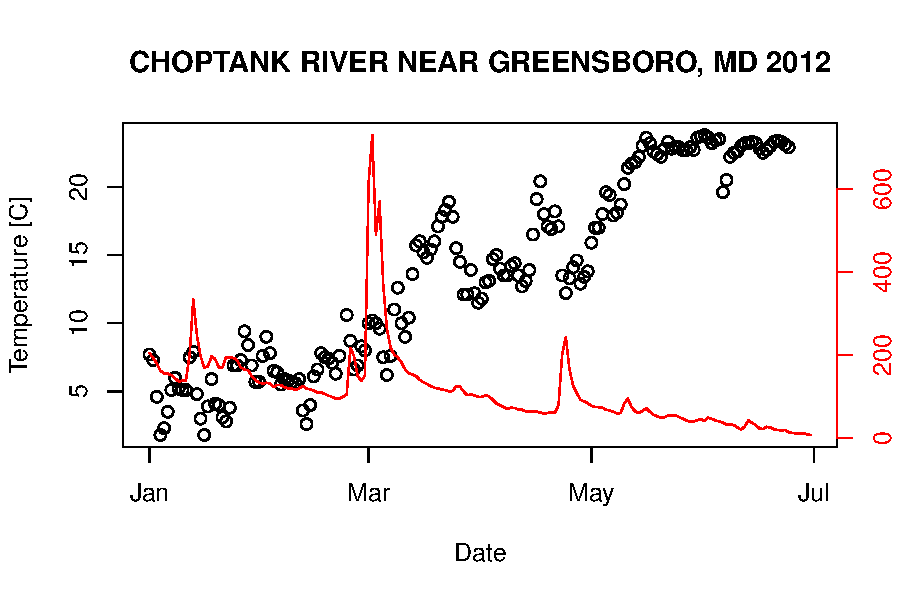
\includegraphics{dataRetrieval-fig1}
\end{center}
\caption{Temperature and discharge plot of Choptank River.}
\end{figure}

There are occasions where NWIS values are not reported as numbers, instead a common example is "Ice".  Any value that cannot be converted to a number will be reported as NA in this package.

%------------------------------------------------------------
\subsection{USGS Unit Value Retrievals}
%------------------------------------------------------------
We can also get real-time, instantaneous measurements using the retrieveUnitNWISData function:
\begin{Schunk}
\begin{Sinput}
> # Using defaults:
> siteNumber <- "01491000" # Site ID for Choptank River near Greensboro, MD
> parameterCd <- "00060"  # Discharge in cubic feet per second
> startDate <- as.character(Sys.Date())
> endDate <- as.character(Sys.Date())
> dischargeToday <- retrieveUnitNWISData(siteNumber, parameterCd, startDate, endDate)